\documentclass[1p]{elsarticle_modified}
%\bibliographystyle{elsarticle-num}

%\usepackage[colorlinks]{hyperref}
%\usepackage{abbrmath_seonhwa} %\Abb, \Ascr, \Acal ,\Abf, \Afrak
\usepackage{amsfonts}
\usepackage{amssymb}
\usepackage{amsmath}
\usepackage{amsthm}
\usepackage{scalefnt}
\usepackage{amsbsy}
\usepackage{kotex}
\usepackage{caption}
\usepackage{subfig}
\usepackage{color}
\usepackage{graphicx}
\usepackage{xcolor} %% white, black, red, green, blue, cyan, magenta, yellow
\usepackage{float}
\usepackage{setspace}
\usepackage{hyperref}

\usepackage{tikz}
\usetikzlibrary{arrows}

\usepackage{multirow}
\usepackage{array} % fixed length table
\usepackage{hhline}

%%%%%%%%%%%%%%%%%%%%%
\makeatletter
\renewcommand*\env@matrix[1][\arraystretch]{%
	\edef\arraystretch{#1}%
	\hskip -\arraycolsep
	\let\@ifnextchar\new@ifnextchar
	\array{*\c@MaxMatrixCols c}}
\makeatother %https://tex.stackexchange.com/questions/14071/how-can-i-increase-the-line-spacing-in-a-matrix
%%%%%%%%%%%%%%%

\usepackage[normalem]{ulem}

\newcommand{\msout}[1]{\ifmmode\text{\sout{\ensuremath{#1}}}\else\sout{#1}\fi}
%SOURCE: \msout is \stkout macro in https://tex.stackexchange.com/questions/20609/strikeout-in-math-mode

\newcommand{\cancel}[1]{
	\ifmmode
	{\color{red}\msout{#1}}
	\else
	{\color{red}\sout{#1}}
	\fi
}

\newcommand{\add}[1]{
	{\color{blue}\uwave{#1}}
}

\newcommand{\replace}[2]{
	\ifmmode
	{\color{red}\msout{#1}}{\color{blue}\uwave{#2}}
	\else
	{\color{red}\sout{#1}}{\color{blue}\uwave{#2}}
	\fi
}

\newcommand{\Sol}{\mathcal{S}} %segment
\newcommand{\D}{D} %diagram
\newcommand{\A}{\mathcal{A}} %arc


%%%%%%%%%%%%%%%%%%%%%%%%%%%%%5 test

\def\sl{\operatorname{\textup{SL}}(2,\Cbb)}
\def\psl{\operatorname{\textup{PSL}}(2,\Cbb)}
\def\quan{\mkern 1mu \triangleright \mkern 1mu}

\theoremstyle{definition}
\newtheorem{thm}{Theorem}[section]
\newtheorem{prop}[thm]{Proposition}
\newtheorem{lem}[thm]{Lemma}
\newtheorem{ques}[thm]{Question}
\newtheorem{cor}[thm]{Corollary}
\newtheorem{defn}[thm]{Definition}
\newtheorem{exam}[thm]{Example}
\newtheorem{rmk}[thm]{Remark}
\newtheorem{alg}[thm]{Algorithm}

\newcommand{\I}{\sqrt{-1}}
\begin{document}

%\begin{frontmatter}
%
%\title{Boundary parabolic representations of knots up to 8 crossings}
%
%%% Group authors per affiliation:
%\author{Yunhi Cho} 
%\address{Department of Mathematics, University of Seoul, Seoul, Korea}
%\ead{yhcho@uos.ac.kr}
%
%
%\author{Seonhwa Kim} %\fnref{s_kim}}
%\address{Center for Geometry and Physics, Institute for Basic Science, Pohang, 37673, Korea}
%\ead{ryeona17@ibs.re.kr}
%
%\author{Hyuk Kim}
%\address{Department of Mathematical Sciences, Seoul National University, Seoul 08826, Korea}
%\ead{hyukkim@snu.ac.kr}
%
%\author{Seokbeom Yoon}
%\address{Department of Mathematical Sciences, Seoul National University, Seoul, 08826,  Korea}
%\ead{sbyoon15@snu.ac.kr}
%
%\begin{abstract}
%We find all boundary parabolic representation of knots up to 8 crossings.
%
%\end{abstract}
%\begin{keyword}
%    \MSC[2010] 57M25 
%\end{keyword}
%
%\end{frontmatter}

%\linenumbers
%\tableofcontents
%
\newcommand\colored[1]{\textcolor{white}{\rule[-0.35ex]{0.8em}{1.4ex}}\kern-0.8em\color{red} #1}%
%\newcommand\colored[1]{\textcolor{white}{ #1}\kern-2.17ex	\textcolor{white}{ #1}\kern-1.81ex	\textcolor{white}{ #1}\kern-2.15ex\color{red}#1	}

{\Large $\underline{12a_{1257}~(K12a_{1257})}$}

\setlength{\tabcolsep}{10pt}
\renewcommand{\arraystretch}{1.6}
\vspace{1cm}\begin{tabular}{m{100pt}>{\centering\arraybackslash}m{274pt}}
\multirow{5}{120pt}{
	\centering
	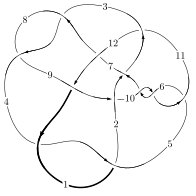
\includegraphics[width=112pt]{../../../GIT/diagram.site/Diagrams/png/2058_12a_1257.png}\\
\ \ \ A knot diagram\footnotemark}&
\allowdisplaybreaks
\textbf{Linearized knot diagam} \\
\cline{2-2}
 &
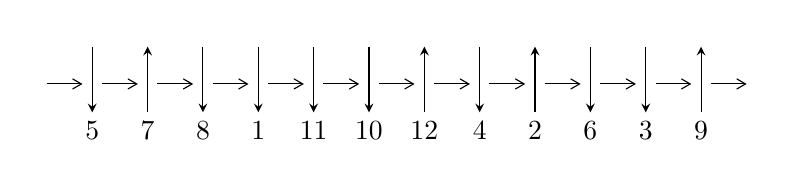
\begin{tikzpicture}[x=20pt, y=17pt]
	% nodes
	\node (C0) at (0, 0) {};
	\node (C1) at (1, 0) {};
	\node (C1U) at (1, +1) {};
	\node (C1D) at (1, -1) {5};

	\node (C2) at (2, 0) {};
	\node (C2U) at (2, +1) {};
	\node (C2D) at (2, -1) {7};

	\node (C3) at (3, 0) {};
	\node (C3U) at (3, +1) {};
	\node (C3D) at (3, -1) {8};

	\node (C4) at (4, 0) {};
	\node (C4U) at (4, +1) {};
	\node (C4D) at (4, -1) {1};

	\node (C5) at (5, 0) {};
	\node (C5U) at (5, +1) {};
	\node (C5D) at (5, -1) {11};

	\node (C6) at (6, 0) {};
	\node (C6U) at (6, +1) {};
	\node (C6D) at (6, -1) {10};

	\node (C7) at (7, 0) {};
	\node (C7U) at (7, +1) {};
	\node (C7D) at (7, -1) {12};

	\node (C8) at (8, 0) {};
	\node (C8U) at (8, +1) {};
	\node (C8D) at (8, -1) {4};

	\node (C9) at (9, 0) {};
	\node (C9U) at (9, +1) {};
	\node (C9D) at (9, -1) {2};

	\node (C10) at (10, 0) {};
	\node (C10U) at (10, +1) {};
	\node (C10D) at (10, -1) {6};

	\node (C11) at (11, 0) {};
	\node (C11U) at (11, +1) {};
	\node (C11D) at (11, -1) {3};

	\node (C12) at (12, 0) {};
	\node (C12U) at (12, +1) {};
	\node (C12D) at (12, -1) {9};
	\node (C13) at (13, 0) {};

	% arrows
	\draw[->,>={angle 60}]
	(C0) edge (C1) (C1) edge (C2) (C2) edge (C3) (C3) edge (C4) (C4) edge (C5) (C5) edge (C6) (C6) edge (C7) (C7) edge (C8) (C8) edge (C9) (C9) edge (C10) (C10) edge (C11) (C11) edge (C12) (C12) edge (C13) ;	\draw[->,>=stealth]
	(C1U) edge (C1D) (C2D) edge (C2U) (C3U) edge (C3D) (C4U) edge (C4D) (C5U) edge (C5D) (C6U) edge (C6D) (C7D) edge (C7U) (C8U) edge (C8D) (C9D) edge (C9U) (C10U) edge (C10D) (C11U) edge (C11D) (C12D) edge (C12U) ;
	\end{tikzpicture} \\
\hhline{~~} \\& 
\textbf{Solving Sequence} \\ \cline{2-2} 
 &
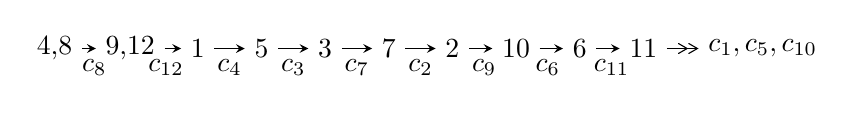
\begin{tikzpicture}[x=23pt, y=7pt]
	% node
	\node (A0) at (-1/8, 0) {4,8};
	\node (A1) at (17/16, 0) {9,12};
	\node (A2) at (17/8, 0) {1};
	\node (A3) at (25/8, 0) {5};
	\node (A4) at (33/8, 0) {3};
	\node (A5) at (41/8, 0) {7};
	\node (A6) at (49/8, 0) {2};
	\node (A7) at (57/8, 0) {10};
	\node (A8) at (65/8, 0) {6};
	\node (A9) at (73/8, 0) {11};
	\node (C1) at (1/2, -1) {$c_{8}$};
	\node (C2) at (13/8, -1) {$c_{12}$};
	\node (C3) at (21/8, -1) {$c_{4}$};
	\node (C4) at (29/8, -1) {$c_{3}$};
	\node (C5) at (37/8, -1) {$c_{7}$};
	\node (C6) at (45/8, -1) {$c_{2}$};
	\node (C7) at (53/8, -1) {$c_{9}$};
	\node (C8) at (61/8, -1) {$c_{6}$};
	\node (C9) at (69/8, -1) {$c_{11}$};
	\node (A10) at (11, 0) {$c_{1},c_{5},c_{10}$};

	% edge
	\draw[->,>=stealth]	
	(A0) edge (A1) (A1) edge (A2) (A2) edge (A3) (A3) edge (A4) (A4) edge (A5) (A5) edge (A6) (A6) edge (A7) (A7) edge (A8) (A8) edge (A9) ;
	\draw[->>,>={angle 60}]	
	(A9) edge (A10);
\end{tikzpicture} \\ 

\end{tabular} \\

\footnotetext{
The image of knot diagram is generated by the software ``\textbf{Draw programme}" developed by Andrew Bartholomew(\url{http://www.layer8.co.uk/maths/draw/index.htm\#Running-draw}), where we modified some parts for our purpose(\url{https://github.com/CATsTAILs/LinksPainter}).
}\phantom \\ \newline 
\centering \textbf{Ideals for irreducible components\footnotemark of $X_{\text{par}}$} 
 
\begin{align*}
I^u_{1}&=\langle 
5.69717\times10^{443} u^{121}-1.08046\times10^{443} u^{120}+\cdots+1.39254\times10^{445} b+1.13421\times10^{446},\\
\phantom{I^u_{1}}&\phantom{= \langle  }-1.11587\times10^{444} u^{121}+9.38471\times10^{444} u^{120}+\cdots+5.98792\times10^{446} a+3.66043\times10^{447},\\
\phantom{I^u_{1}}&\phantom{= \langle  }u^{122}- u^{121}+\cdots+840 u-344\rangle \\
I^u_{2}&=\langle 
24839975132 u^{20}+42789429212 u^{19}+\cdots+64008861027 b-50213545124,\\
\phantom{I^u_{2}}&\phantom{= \langle  }44188587683 u^{20}+143099664266 u^{19}+\cdots+64008861027 a-168032991365,\\
\phantom{I^u_{2}}&\phantom{= \langle  }u^{21}-7 u^{19}+\cdots-5 u^2+1\rangle \\
\\
\end{align*}
\raggedright * 2 irreducible components of $\dim_{\mathbb{C}}=0$, with total 143 representations.\\
\footnotetext{All coefficients of polynomials are rational numbers. But the coefficients are sometimes approximated in decimal forms when there is not enough margin.}
\newpage
\renewcommand{\arraystretch}{1}
\centering \section*{I. $I^u_{1}= \langle 5.70\times10^{443} u^{121}-1.08\times10^{443} u^{120}+\cdots+1.39\times10^{445} b+1.13\times10^{446},\;-1.12\times10^{444} u^{121}+9.38\times10^{444} u^{120}+\cdots+5.99\times10^{446} a+3.66\times10^{447},\;u^{122}- u^{121}+\cdots+840 u-344 \rangle$}
\flushleft \textbf{(i) Arc colorings}\\
\begin{tabular}{m{7pt} m{180pt} m{7pt} m{180pt} }
\flushright $a_{4}=$&$\begin{pmatrix}0\\u\end{pmatrix}$ \\
\flushright $a_{8}=$&$\begin{pmatrix}1\\0\end{pmatrix}$ \\
\flushright $a_{9}=$&$\begin{pmatrix}1\\u^2\end{pmatrix}$ \\
\flushright $a_{12}=$&$\begin{pmatrix}0.00186353 u^{121}-0.0156727 u^{120}+\cdots+8.69189 u-6.11302\\-0.0409121 u^{121}+0.00775889 u^{120}+\cdots+10.8209 u-8.14493\end{pmatrix}$ \\
\flushright $a_{1}=$&$\begin{pmatrix}-0.0424622 u^{121}+0.0182287 u^{120}+\cdots+7.27198 u-9.50758\\-0.0988281 u^{121}+0.0548574 u^{120}+\cdots+4.32925 u-11.7309\end{pmatrix}$ \\
\flushright $a_{5}=$&$\begin{pmatrix}-0.0333642 u^{121}+0.00722217 u^{120}+\cdots+9.88193 u-10.3188\\-0.0518144 u^{121}-0.0133058 u^{120}+\cdots+31.5122 u-17.0446\end{pmatrix}$ \\
\flushright $a_{3}=$&$\begin{pmatrix}u\\u\end{pmatrix}$ \\
\flushright $a_{7}=$&$\begin{pmatrix}0.0249558 u^{121}+0.0248564 u^{120}+\cdots-22.7064 u+12.6805\\0.0259868 u^{121}+0.0332605 u^{120}+\cdots-28.4800 u+14.2995\end{pmatrix}$ \\
\flushright $a_{2}=$&$\begin{pmatrix}0.0790093 u^{121}-0.0280193 u^{120}+\cdots+9.57936 u+9.70489\\0.104578 u^{121}-0.0400487 u^{120}+\cdots-11.8432 u+17.6024\end{pmatrix}$ \\
\flushright $a_{10}=$&$\begin{pmatrix}-0.0567863 u^{121}-0.0247468 u^{120}+\cdots+25.8798 u-21.9604\\-0.0657310 u^{121}-0.0362288 u^{120}+\cdots+51.9703 u-29.6219\end{pmatrix}$ \\
\flushright $a_{6}=$&$\begin{pmatrix}-0.0178133 u^{121}+0.0149639 u^{120}+\cdots+3.63656 u-4.43187\\-0.00460256 u^{121}+0.0149540 u^{120}+\cdots-4.51681 u+3.76614\end{pmatrix}$ \\
\flushright $a_{11}=$&$\begin{pmatrix}-0.0565800 u^{121}+0.0189299 u^{120}+\cdots+10.2260 u-12.7674\\-0.0993556 u^{121}+0.0423615 u^{120}+\cdots+12.3550 u-14.7993\end{pmatrix}$\\&\end{tabular}
\flushleft \textbf{(ii) Obstruction class $= -1$}\\~\\
\flushleft \textbf{(iii) Cusp Shapes $= 0.0488883 u^{121}+0.0908826 u^{120}+\cdots-102.646 u+42.5994$}\\~\\
\newpage\renewcommand{\arraystretch}{1}
\flushleft \textbf{(iv) u-Polynomials at the component}\newline \\
\begin{tabular}{m{50pt}|m{274pt}}
Crossings & \hspace{64pt}u-Polynomials at each crossing \\
\hline $$\begin{aligned}c_{1},c_{4}\end{aligned}$$&$\begin{aligned}
&3(3 u^{122}+10 u^{121}+\cdots+187864 u+5572)
\end{aligned}$\\
\hline $$\begin{aligned}c_{2}\end{aligned}$$&$\begin{aligned}
&3(3 u^{122}-4 u^{121}+\cdots-1118665 u-446825)
\end{aligned}$\\
\hline $$\begin{aligned}c_{3},c_{8}\end{aligned}$$&$\begin{aligned}
&u^{122}- u^{121}+\cdots+840 u-344
\end{aligned}$\\
\hline $$\begin{aligned}c_{5},c_{6},c_{10}\end{aligned}$$&$\begin{aligned}
&u^{122}+u^{121}+\cdots+8 u-11
\end{aligned}$\\
\hline $$\begin{aligned}c_{7}\end{aligned}$$&$\begin{aligned}
&3(3 u^{122}-7 u^{121}+\cdots-2 u+1)
\end{aligned}$\\
\hline $$\begin{aligned}c_{9}\end{aligned}$$&$\begin{aligned}
&u^{122}-2 u^{121}+\cdots+950272 u-49152
\end{aligned}$\\
\hline $$\begin{aligned}c_{11}\end{aligned}$$&$\begin{aligned}
&u^{122}+4 u^{121}+\cdots+111658 u-20519
\end{aligned}$\\
\hline $$\begin{aligned}c_{12}\end{aligned}$$&$\begin{aligned}
&u^{122}-3 u^{121}+\cdots+51487 u-8787
\end{aligned}$\\
\hline
\end{tabular}\\~\\
\newpage\renewcommand{\arraystretch}{1}
\flushleft \textbf{(v) Riley Polynomials at the component}\newline \\
\begin{tabular}{m{50pt}|m{274pt}}
Crossings & \hspace{64pt}Riley Polynomials at each crossing \\
\hline $$\begin{aligned}c_{1},c_{4}\end{aligned}$$&$\begin{aligned}
&9(9 y^{122}-898 y^{121}+\cdots-7.94711\times10^{9} y+3.10472\times10^{7})
\end{aligned}$\\
\hline $$\begin{aligned}c_{2}\end{aligned}$$&$\begin{aligned}
&9(9 y^{122}-388 y^{121}+\cdots-2.27562\times10^{12} y+1.99653\times10^{11})
\end{aligned}$\\
\hline $$\begin{aligned}c_{3},c_{8}\end{aligned}$$&$\begin{aligned}
&y^{122}-91 y^{121}+\cdots-740000 y+118336
\end{aligned}$\\
\hline $$\begin{aligned}c_{5},c_{6},c_{10}\end{aligned}$$&$\begin{aligned}
&y^{122}+115 y^{121}+\cdots-8600 y+121
\end{aligned}$\\
\hline $$\begin{aligned}c_{7}\end{aligned}$$&$\begin{aligned}
&9(9 y^{122}+5 y^{121}+\cdots-20 y+1)
\end{aligned}$\\
\hline $$\begin{aligned}c_{9}\end{aligned}$$&$\begin{aligned}
&y^{122}-22 y^{121}+\cdots-561164320768 y+2415919104
\end{aligned}$\\
\hline $$\begin{aligned}c_{11}\end{aligned}$$&$\begin{aligned}
&y^{122}-14 y^{121}+\cdots-28711211162 y+421029361
\end{aligned}$\\
\hline $$\begin{aligned}c_{12}\end{aligned}$$&$\begin{aligned}
&y^{122}+53 y^{121}+\cdots+2230478219 y+77211369
\end{aligned}$\\
\hline
\end{tabular}\\~\\
\newpage\flushleft \textbf{(vi) Complex Volumes and Cusp Shapes}
$$\begin{array}{c|c|c}  
\text{Solutions to }I^u_{1}& \I (\text{vol} + \sqrt{-1}CS) & \text{Cusp shape}\\
 \hline 
\begin{aligned}
u &= \phantom{-}0.604012 + 0.787190 I \\
a &= \phantom{-}1.151760 - 0.060842 I \\
b &= -0.862030 + 0.023194 I\end{aligned}
 & \phantom{-}4.52117 + 4.07559 I & \phantom{-0.000000 } 0 \\ \hline\begin{aligned}
u &= \phantom{-}0.604012 - 0.787190 I \\
a &= \phantom{-}1.151760 + 0.060842 I \\
b &= -0.862030 - 0.023194 I\end{aligned}
 & \phantom{-}4.52117 - 4.07559 I & \phantom{-0.000000 } 0 \\ \hline\begin{aligned}
u &= \phantom{-}1.000660 + 0.207886 I \\
a &= -0.436527 + 1.299170 I \\
b &= -0.235979 + 0.305966 I\end{aligned}
 & \phantom{-}0.36555 - 2.39525 I & \phantom{-0.000000 } 0 \\ \hline\begin{aligned}
u &= \phantom{-}1.000660 - 0.207886 I \\
a &= -0.436527 - 1.299170 I \\
b &= -0.235979 - 0.305966 I\end{aligned}
 & \phantom{-}0.36555 + 2.39525 I & \phantom{-0.000000 } 0 \\ \hline\begin{aligned}
u &= \phantom{-}0.976833 + 0.387500 I \\
a &= -0.62050 - 1.97893 I \\
b &= \phantom{-}0.354146 - 0.011955 I\end{aligned}
 & \phantom{-}3.34528 - 8.66044 I & \phantom{-0.000000 } 0 \\ \hline\begin{aligned}
u &= \phantom{-}0.976833 - 0.387500 I \\
a &= -0.62050 + 1.97893 I \\
b &= \phantom{-}0.354146 + 0.011955 I\end{aligned}
 & \phantom{-}3.34528 + 8.66044 I & \phantom{-0.000000 } 0 \\ \hline\begin{aligned}
u &= -0.240514 + 0.903459 I \\
a &= -0.106658 + 0.239405 I \\
b &= \phantom{-}0.937678 + 0.678854 I\end{aligned}
 & \phantom{-}0.12332 + 4.01287 I & \phantom{-0.000000 } 0 \\ \hline\begin{aligned}
u &= -0.240514 - 0.903459 I \\
a &= -0.106658 - 0.239405 I \\
b &= \phantom{-}0.937678 - 0.678854 I\end{aligned}
 & \phantom{-}0.12332 - 4.01287 I & \phantom{-0.000000 } 0 \\ \hline\begin{aligned}
u &= -0.136181 + 0.916927 I \\
a &= \phantom{-}0.155274 + 0.361001 I \\
b &= \phantom{-}0.930982 - 0.743513 I\end{aligned}
 & \phantom{-}8.57001 - 7.32077 I & \phantom{-0.000000 } 0 \\ \hline\begin{aligned}
u &= -0.136181 - 0.916927 I \\
a &= \phantom{-}0.155274 - 0.361001 I \\
b &= \phantom{-}0.930982 + 0.743513 I\end{aligned}
 & \phantom{-}8.57001 + 7.32077 I & \phantom{-0.000000 } 0\\
 \hline 
 \end{array}$$\newpage$$\begin{array}{c|c|c}  
\text{Solutions to }I^u_{1}& \I (\text{vol} + \sqrt{-1}CS) & \text{Cusp shape}\\
 \hline 
\begin{aligned}
u &= -0.966501 + 0.499176 I \\
a &= -0.666110 + 0.332942 I \\
b &= -0.423485 + 0.385406 I\end{aligned}
 & -1.79362 + 0.74361 I & \phantom{-0.000000 } 0 \\ \hline\begin{aligned}
u &= -0.966501 - 0.499176 I \\
a &= -0.666110 - 0.332942 I \\
b &= -0.423485 - 0.385406 I\end{aligned}
 & -1.79362 - 0.74361 I & \phantom{-0.000000 } 0 \\ \hline\begin{aligned}
u &= -0.867098 + 0.253936 I \\
a &= \phantom{-}0.61988 + 1.94729 I \\
b &= \phantom{-}0.457387 + 0.092056 I\end{aligned}
 & \phantom{-}7.08067 + 3.95400 I & \phantom{-0.000000 } 0 \\ \hline\begin{aligned}
u &= -0.867098 - 0.253936 I \\
a &= \phantom{-}0.61988 - 1.94729 I \\
b &= \phantom{-}0.457387 - 0.092056 I\end{aligned}
 & \phantom{-}7.08067 - 3.95400 I & \phantom{-0.000000 } 0 \\ \hline\begin{aligned}
u &= -0.088634 + 0.886156 I \\
a &= \phantom{-}0.293338 + 0.175849 I \\
b &= -0.952380 + 0.636078 I\end{aligned}
 & \phantom{-}7.63214 - 1.85396 I & \phantom{-0.000000 } 0 \\ \hline\begin{aligned}
u &= -0.088634 - 0.886156 I \\
a &= \phantom{-}0.293338 - 0.175849 I \\
b &= -0.952380 - 0.636078 I\end{aligned}
 & \phantom{-}7.63214 + 1.85396 I & \phantom{-0.000000 } 0 \\ \hline\begin{aligned}
u &= \phantom{-}1.084380 + 0.239590 I \\
a &= \phantom{-}1.03058 + 1.77666 I \\
b &= \phantom{-}0.55960 + 2.00322 I\end{aligned}
 & \phantom{-}2.71157 + 0.31538 I & \phantom{-0.000000 } 0 \\ \hline\begin{aligned}
u &= \phantom{-}1.084380 - 0.239590 I \\
a &= \phantom{-}1.03058 - 1.77666 I \\
b &= \phantom{-}0.55960 - 2.00322 I\end{aligned}
 & \phantom{-}2.71157 - 0.31538 I & \phantom{-0.000000 } 0 \\ \hline\begin{aligned}
u &= \phantom{-}1.122500 + 0.217741 I \\
a &= \phantom{-}0.70445 - 1.89025 I \\
b &= \phantom{-}1.32380 - 1.19693 I\end{aligned}
 & \phantom{-}5.88182 - 0.15056 I & \phantom{-0.000000 } 0 \\ \hline\begin{aligned}
u &= \phantom{-}1.122500 - 0.217741 I \\
a &= \phantom{-}0.70445 + 1.89025 I \\
b &= \phantom{-}1.32380 + 1.19693 I\end{aligned}
 & \phantom{-}5.88182 + 0.15056 I & \phantom{-0.000000 } 0\\
 \hline 
 \end{array}$$\newpage$$\begin{array}{c|c|c}  
\text{Solutions to }I^u_{1}& \I (\text{vol} + \sqrt{-1}CS) & \text{Cusp shape}\\
 \hline 
\begin{aligned}
u &= \phantom{-}1.146260 + 0.042855 I \\
a &= -0.582703 + 0.076661 I \\
b &= -1.88629 - 0.09036 I\end{aligned}
 & \phantom{-}0.189968 - 1.251570 I & \phantom{-0.000000 } 0 \\ \hline\begin{aligned}
u &= \phantom{-}1.146260 - 0.042855 I \\
a &= -0.582703 - 0.076661 I \\
b &= -1.88629 + 0.09036 I\end{aligned}
 & \phantom{-}0.189968 + 1.251570 I & \phantom{-0.000000 } 0 \\ \hline\begin{aligned}
u &= \phantom{-}0.290670 + 1.111480 I \\
a &= \phantom{-}0.087173 + 0.145864 I \\
b &= -0.903371 + 0.688115 I\end{aligned}
 & -1.01392 - 8.75038 I & \phantom{-0.000000 } 0 \\ \hline\begin{aligned}
u &= \phantom{-}0.290670 - 1.111480 I \\
a &= \phantom{-}0.087173 - 0.145864 I \\
b &= -0.903371 - 0.688115 I\end{aligned}
 & -1.01392 + 8.75038 I & \phantom{-0.000000 } 0 \\ \hline\begin{aligned}
u &= -1.14892\phantom{ +0.000000I} \\
a &= \phantom{-}0.659162\phantom{ +0.000000I} \\
b &= \phantom{-}1.89148\phantom{ +0.000000I}\end{aligned}
 & -4.37114\phantom{ +0.000000I} & \phantom{-0.000000 } 0 \\ \hline\begin{aligned}
u &= -1.138110 + 0.195030 I \\
a &= -0.15246 + 1.76125 I \\
b &= \phantom{-}0.61079 + 1.57952 I\end{aligned}
 & -3.14459 + 1.16883 I & \phantom{-0.000000 } 0 \\ \hline\begin{aligned}
u &= -1.138110 - 0.195030 I \\
a &= -0.15246 - 1.76125 I \\
b &= \phantom{-}0.61079 - 1.57952 I\end{aligned}
 & -3.14459 - 1.16883 I & \phantom{-0.000000 } 0 \\ \hline\begin{aligned}
u &= \phantom{-}0.007461 + 0.835751 I \\
a &= -0.073744 + 0.397542 I \\
b &= -0.890083 - 0.595912 I\end{aligned}
 & \phantom{-}2.55112 + 4.21322 I & \phantom{-0.000000 } 0 \\ \hline\begin{aligned}
u &= \phantom{-}0.007461 - 0.835751 I \\
a &= -0.073744 - 0.397542 I \\
b &= -0.890083 + 0.595912 I\end{aligned}
 & \phantom{-}2.55112 - 4.21322 I & \phantom{-0.000000 } 0 \\ \hline\begin{aligned}
u &= \phantom{-}1.179670 + 0.033463 I \\
a &= -0.97750 - 1.76730 I \\
b &= \phantom{-}0.740671 - 0.709642 I\end{aligned}
 & \phantom{-}0.69055 - 7.86145 I & \phantom{-0.000000 } 0\\
 \hline 
 \end{array}$$\newpage$$\begin{array}{c|c|c}  
\text{Solutions to }I^u_{1}& \I (\text{vol} + \sqrt{-1}CS) & \text{Cusp shape}\\
 \hline 
\begin{aligned}
u &= \phantom{-}1.179670 - 0.033463 I \\
a &= -0.97750 + 1.76730 I \\
b &= \phantom{-}0.740671 + 0.709642 I\end{aligned}
 & \phantom{-}0.69055 + 7.86145 I & \phantom{-0.000000 } 0 \\ \hline\begin{aligned}
u &= -1.187310 + 0.055707 I \\
a &= \phantom{-}0.57715 + 2.43247 I \\
b &= -0.392933 + 0.907576 I\end{aligned}
 & -5.78046 - 2.67801 I & \phantom{-0.000000 } 0 \\ \hline\begin{aligned}
u &= -1.187310 - 0.055707 I \\
a &= \phantom{-}0.57715 - 2.43247 I \\
b &= -0.392933 - 0.907576 I\end{aligned}
 & -5.78046 + 2.67801 I & \phantom{-0.000000 } 0 \\ \hline\begin{aligned}
u &= -1.171740 + 0.243574 I \\
a &= -0.48719 - 1.83317 I \\
b &= -0.100075 - 0.249733 I\end{aligned}
 & -4.23137 + 5.27335 I & \phantom{-0.000000 } 0 \\ \hline\begin{aligned}
u &= -1.171740 - 0.243574 I \\
a &= -0.48719 + 1.83317 I \\
b &= -0.100075 + 0.249733 I\end{aligned}
 & -4.23137 - 5.27335 I & \phantom{-0.000000 } 0 \\ \hline\begin{aligned}
u &= \phantom{-}1.208310 + 0.188282 I \\
a &= \phantom{-}0.08160 + 2.47331 I \\
b &= -0.241048 + 1.103970 I\end{aligned}
 & -4.88247 - 3.91427 I & \phantom{-0.000000 } 0 \\ \hline\begin{aligned}
u &= \phantom{-}1.208310 - 0.188282 I \\
a &= \phantom{-}0.08160 - 2.47331 I \\
b &= -0.241048 - 1.103970 I\end{aligned}
 & -4.88247 + 3.91427 I & \phantom{-0.000000 } 0 \\ \hline\begin{aligned}
u &= -0.687999 + 0.359730 I \\
a &= \phantom{-}0.848366 - 0.061263 I \\
b &= -1.153990 + 0.002434 I\end{aligned}
 & \phantom{-}7.72907 - 1.13566 I & \phantom{-0.000000 } 0 \\ \hline\begin{aligned}
u &= -0.687999 - 0.359730 I \\
a &= \phantom{-}0.848366 + 0.061263 I \\
b &= -1.153990 - 0.002434 I\end{aligned}
 & \phantom{-}7.72907 + 1.13566 I & \phantom{-0.000000 } 0 \\ \hline\begin{aligned}
u &= -0.303172 + 0.711246 I \\
a &= -1.059850 - 0.757480 I \\
b &= \phantom{-}0.725735 - 0.022937 I\end{aligned}
 & -1.45418 - 1.75021 I & \phantom{-0.000000 } 0\\
 \hline 
 \end{array}$$\newpage$$\begin{array}{c|c|c}  
\text{Solutions to }I^u_{1}& \I (\text{vol} + \sqrt{-1}CS) & \text{Cusp shape}\\
 \hline 
\begin{aligned}
u &= -0.303172 - 0.711246 I \\
a &= -1.059850 + 0.757480 I \\
b &= \phantom{-}0.725735 + 0.022937 I\end{aligned}
 & -1.45418 + 1.75021 I & \phantom{-0.000000 } 0 \\ \hline\begin{aligned}
u &= \phantom{-}1.194850 + 0.297888 I \\
a &= \phantom{-}0.26968 + 1.47503 I \\
b &= -0.762477 + 0.986963 I\end{aligned}
 & -3.44043 - 4.18263 I & \phantom{-0.000000 } 0 \\ \hline\begin{aligned}
u &= \phantom{-}1.194850 - 0.297888 I \\
a &= \phantom{-}0.26968 - 1.47503 I \\
b &= -0.762477 - 0.986963 I\end{aligned}
 & -3.44043 + 4.18263 I & \phantom{-0.000000 } 0 \\ \hline\begin{aligned}
u &= -1.174990 + 0.399163 I \\
a &= -0.64210 + 1.40000 I \\
b &= \phantom{-}0.835123 + 0.753703 I\end{aligned}
 & \phantom{-}2.92338 + 6.99742 I & \phantom{-0.000000 } 0 \\ \hline\begin{aligned}
u &= -1.174990 - 0.399163 I \\
a &= -0.64210 - 1.40000 I \\
b &= \phantom{-}0.835123 - 0.753703 I\end{aligned}
 & \phantom{-}2.92338 - 6.99742 I & \phantom{-0.000000 } 0 \\ \hline\begin{aligned}
u &= -1.241760 + 0.061173 I \\
a &= -0.76484 + 1.83008 I \\
b &= -1.07189 + 1.57808 I\end{aligned}
 & -5.21797 - 0.40787 I & \phantom{-0.000000 } 0 \\ \hline\begin{aligned}
u &= -1.241760 - 0.061173 I \\
a &= -0.76484 - 1.83008 I \\
b &= -1.07189 - 1.57808 I\end{aligned}
 & -5.21797 + 0.40787 I & \phantom{-0.000000 } 0 \\ \hline\begin{aligned}
u &= \phantom{-}1.25518\phantom{ +0.000000I} \\
a &= \phantom{-}1.40422\phantom{ +0.000000I} \\
b &= -0.230257\phantom{ +0.000000I}\end{aligned}
 & -6.77287\phantom{ +0.000000I} & \phantom{-0.000000 } 0 \\ \hline\begin{aligned}
u &= -0.236158 + 1.234460 I \\
a &= -0.100891 + 0.105992 I \\
b &= \phantom{-}0.890900 + 0.723943 I\end{aligned}
 & \phantom{-}4.87949 + 12.70870 I & \phantom{-0.000000 } 0 \\ \hline\begin{aligned}
u &= -0.236158 - 1.234460 I \\
a &= -0.100891 - 0.105992 I \\
b &= \phantom{-}0.890900 - 0.723943 I\end{aligned}
 & \phantom{-}4.87949 - 12.70870 I & \phantom{-0.000000 } 0\\
 \hline 
 \end{array}$$\newpage$$\begin{array}{c|c|c}  
\text{Solutions to }I^u_{1}& \I (\text{vol} + \sqrt{-1}CS) & \text{Cusp shape}\\
 \hline 
\begin{aligned}
u &= -1.246630 + 0.255267 I \\
a &= \phantom{-}0.172527 - 0.247100 I \\
b &= \phantom{-}1.051920 - 0.043007 I\end{aligned}
 & -3.43189 + 3.95846 I & \phantom{-0.000000 } 0 \\ \hline\begin{aligned}
u &= -1.246630 - 0.255267 I \\
a &= \phantom{-}0.172527 + 0.247100 I \\
b &= \phantom{-}1.051920 + 0.043007 I\end{aligned}
 & -3.43189 - 3.95846 I & \phantom{-0.000000 } 0 \\ \hline\begin{aligned}
u &= \phantom{-}1.273820 + 0.112467 I \\
a &= \phantom{-}0.57249 + 1.66884 I \\
b &= \phantom{-}1.00345 + 1.58304 I\end{aligned}
 & -7.11559 - 5.13445 I & \phantom{-0.000000 } 0 \\ \hline\begin{aligned}
u &= \phantom{-}1.273820 - 0.112467 I \\
a &= \phantom{-}0.57249 - 1.66884 I \\
b &= \phantom{-}1.00345 - 1.58304 I\end{aligned}
 & -7.11559 + 5.13445 I & \phantom{-0.000000 } 0 \\ \hline\begin{aligned}
u &= -1.255070 + 0.273667 I \\
a &= -0.53404 - 1.58140 I \\
b &= -1.29853 - 1.19048 I\end{aligned}
 & -1.26423 + 3.63180 I & \phantom{-0.000000 } 0 \\ \hline\begin{aligned}
u &= -1.255070 - 0.273667 I \\
a &= -0.53404 + 1.58140 I \\
b &= -1.29853 + 1.19048 I\end{aligned}
 & -1.26423 - 3.63180 I & \phantom{-0.000000 } 0 \\ \hline\begin{aligned}
u &= -1.275990 + 0.166531 I \\
a &= \phantom{-}0.119660 - 0.202339 I \\
b &= -0.290527 - 0.199626 I\end{aligned}
 & -1.78102 + 0.04002 I & \phantom{-0.000000 } 0 \\ \hline\begin{aligned}
u &= -1.275990 - 0.166531 I \\
a &= \phantom{-}0.119660 + 0.202339 I \\
b &= -0.290527 + 0.199626 I\end{aligned}
 & -1.78102 - 0.04002 I & \phantom{-0.000000 } 0 \\ \hline\begin{aligned}
u &= -1.294610 + 0.150957 I \\
a &= -0.56206 + 1.51842 I \\
b &= -1.03035 + 1.61105 I\end{aligned}
 & -1.27716 + 9.56420 I & \phantom{-0.000000 } 0 \\ \hline\begin{aligned}
u &= -1.294610 - 0.150957 I \\
a &= -0.56206 - 1.51842 I \\
b &= -1.03035 - 1.61105 I\end{aligned}
 & -1.27716 - 9.56420 I & \phantom{-0.000000 } 0\\
 \hline 
 \end{array}$$\newpage$$\begin{array}{c|c|c}  
\text{Solutions to }I^u_{1}& \I (\text{vol} + \sqrt{-1}CS) & \text{Cusp shape}\\
 \hline 
\begin{aligned}
u &= -1.230320 + 0.437781 I \\
a &= -0.13075 - 1.65724 I \\
b &= -1.25919 - 1.31101 I\end{aligned}
 & \phantom{-}5.14389 + 12.14870 I & \phantom{-0.000000 } 0 \\ \hline\begin{aligned}
u &= -1.230320 - 0.437781 I \\
a &= -0.13075 + 1.65724 I \\
b &= -1.25919 + 1.31101 I\end{aligned}
 & \phantom{-}5.14389 - 12.14870 I & \phantom{-0.000000 } 0 \\ \hline\begin{aligned}
u &= \phantom{-}1.312370 + 0.071022 I \\
a &= -0.133076 - 0.649670 I \\
b &= -1.031410 - 0.530995 I\end{aligned}
 & -7.22586 - 0.26019 I & \phantom{-0.000000 } 0 \\ \hline\begin{aligned}
u &= \phantom{-}1.312370 - 0.071022 I \\
a &= -0.133076 + 0.649670 I \\
b &= -1.031410 + 0.530995 I\end{aligned}
 & -7.22586 + 0.26019 I & \phantom{-0.000000 } 0 \\ \hline\begin{aligned}
u &= -1.245050 + 0.427250 I \\
a &= -0.07700 + 1.74458 I \\
b &= \phantom{-}0.934702 + 0.941172 I\end{aligned}
 & \phantom{-}4.03093 + 6.55649 I & \phantom{-0.000000 } 0 \\ \hline\begin{aligned}
u &= -1.245050 - 0.427250 I \\
a &= -0.07700 - 1.74458 I \\
b &= \phantom{-}0.934702 - 0.941172 I\end{aligned}
 & \phantom{-}4.03093 - 6.55649 I & \phantom{-0.000000 } 0 \\ \hline\begin{aligned}
u &= \phantom{-}0.103787 + 1.318050 I \\
a &= \phantom{-}0.265587 - 0.229174 I \\
b &= -0.550013 - 0.296741 I\end{aligned}
 & \phantom{-}0.549767 + 1.184870 I & \phantom{-0.000000 } 0 \\ \hline\begin{aligned}
u &= \phantom{-}0.103787 - 1.318050 I \\
a &= \phantom{-}0.265587 + 0.229174 I \\
b &= -0.550013 + 0.296741 I\end{aligned}
 & \phantom{-}0.549767 - 1.184870 I & \phantom{-0.000000 } 0 \\ \hline\begin{aligned}
u &= \phantom{-}1.268610 + 0.377816 I \\
a &= \phantom{-}0.27334 - 1.56476 I \\
b &= \phantom{-}1.24182 - 1.24543 I\end{aligned}
 & -1.37091 - 8.56529 I & \phantom{-0.000000 } 0 \\ \hline\begin{aligned}
u &= \phantom{-}1.268610 - 0.377816 I \\
a &= \phantom{-}0.27334 + 1.56476 I \\
b &= \phantom{-}1.24182 + 1.24543 I\end{aligned}
 & -1.37091 + 8.56529 I & \phantom{-0.000000 } 0\\
 \hline 
 \end{array}$$\newpage$$\begin{array}{c|c|c}  
\text{Solutions to }I^u_{1}& \I (\text{vol} + \sqrt{-1}CS) & \text{Cusp shape}\\
 \hline 
\begin{aligned}
u &= \phantom{-}0.645612 + 0.061796 I \\
a &= \phantom{-}2.74885 + 0.68647 I \\
b &= \phantom{-}1.180570 + 0.241608 I\end{aligned}
 & \phantom{-}2.01963 - 1.05555 I & -12.10339 + 2.04316 I \\ \hline\begin{aligned}
u &= \phantom{-}0.645612 - 0.061796 I \\
a &= \phantom{-}2.74885 - 0.68647 I \\
b &= \phantom{-}1.180570 - 0.241608 I\end{aligned}
 & \phantom{-}2.01963 + 1.05555 I & -12.10339 - 2.04316 I \\ \hline\begin{aligned}
u &= -1.352450 + 0.066592 I \\
a &= \phantom{-}0.087455 + 0.980535 I \\
b &= \phantom{-}1.049130 + 0.936651 I\end{aligned}
 & -3.39022 + 2.98405 I & \phantom{-0.000000 } 0 \\ \hline\begin{aligned}
u &= -1.352450 - 0.066592 I \\
a &= \phantom{-}0.087455 - 0.980535 I \\
b &= \phantom{-}1.049130 - 0.936651 I\end{aligned}
 & -3.39022 - 2.98405 I & \phantom{-0.000000 } 0 \\ \hline\begin{aligned}
u &= -0.110309 + 0.572008 I \\
a &= \phantom{-}1.229000 - 0.416576 I \\
b &= -0.347171 + 0.793115 I\end{aligned}
 & \phantom{-}5.91854 - 3.13751 I & \phantom{-}0.76663 + 1.77568 I \\ \hline\begin{aligned}
u &= -0.110309 - 0.572008 I \\
a &= \phantom{-}1.229000 + 0.416576 I \\
b &= -0.347171 - 0.793115 I\end{aligned}
 & \phantom{-}5.91854 + 3.13751 I & \phantom{-}0.76663 - 1.77568 I \\ \hline\begin{aligned}
u &= \phantom{-}0.068199 + 0.544487 I \\
a &= -0.103221 + 0.664665 I \\
b &= \phantom{-}1.034830 - 0.343908 I\end{aligned}
 & \phantom{-}2.70887 - 0.48608 I & \phantom{-}3.14941 - 1.48071 I \\ \hline\begin{aligned}
u &= \phantom{-}0.068199 - 0.544487 I \\
a &= -0.103221 - 0.664665 I \\
b &= \phantom{-}1.034830 + 0.343908 I\end{aligned}
 & \phantom{-}2.70887 + 0.48608 I & \phantom{-}3.14941 + 1.48071 I \\ \hline\begin{aligned}
u &= \phantom{-}1.40814 + 0.41089 I \\
a &= -0.18904 + 1.63083 I \\
b &= -1.09729 + 1.16633 I\end{aligned}
 & -5.04061 - 8.77658 I & \phantom{-0.000000 } 0 \\ \hline\begin{aligned}
u &= \phantom{-}1.40814 - 0.41089 I \\
a &= -0.18904 - 1.63083 I \\
b &= -1.09729 - 1.16633 I\end{aligned}
 & -5.04061 + 8.77658 I & \phantom{-0.000000 } 0\\
 \hline 
 \end{array}$$\newpage$$\begin{array}{c|c|c}  
\text{Solutions to }I^u_{1}& \I (\text{vol} + \sqrt{-1}CS) & \text{Cusp shape}\\
 \hline 
\begin{aligned}
u &= \phantom{-}0.285251 + 0.447657 I \\
a &= -0.469896 + 0.646478 I \\
b &= -1.316700 - 0.502443 I\end{aligned}
 & \phantom{-}8.41814 - 2.55121 I & \phantom{-}4.33699 + 5.44008 I \\ \hline\begin{aligned}
u &= \phantom{-}0.285251 - 0.447657 I \\
a &= -0.469896 - 0.646478 I \\
b &= -1.316700 + 0.502443 I\end{aligned}
 & \phantom{-}8.41814 + 2.55121 I & \phantom{-}4.33699 - 5.44008 I \\ \hline\begin{aligned}
u &= \phantom{-}0.351099 + 0.371932 I \\
a &= \phantom{-}2.26061 - 0.65659 I \\
b &= \phantom{-}0.452952 + 0.854468 I\end{aligned}
 & \phantom{-}1.94986 - 1.37190 I & -3.76005 - 3.82007 I \\ \hline\begin{aligned}
u &= \phantom{-}0.351099 - 0.371932 I \\
a &= \phantom{-}2.26061 + 0.65659 I \\
b &= \phantom{-}0.452952 - 0.854468 I\end{aligned}
 & \phantom{-}1.94986 + 1.37190 I & -3.76005 + 3.82007 I \\ \hline\begin{aligned}
u &= -1.43663 + 0.39328 I \\
a &= -0.018429 - 1.154060 I \\
b &= -0.290989 - 0.943659 I\end{aligned}
 & -5.43258 + 4.56786 I & \phantom{-0.000000 } 0 \\ \hline\begin{aligned}
u &= -1.43663 - 0.39328 I \\
a &= -0.018429 + 1.154060 I \\
b &= -0.290989 + 0.943659 I\end{aligned}
 & -5.43258 - 4.56786 I & \phantom{-0.000000 } 0 \\ \hline\begin{aligned}
u &= \phantom{-}1.09205 + 1.01974 I \\
a &= -0.0585516 + 0.0289578 I \\
b &= \phantom{-}0.309304 - 0.236222 I\end{aligned}
 & \phantom{-}2.12157 - 3.07632 I & \phantom{-0.000000 } 0 \\ \hline\begin{aligned}
u &= \phantom{-}1.09205 - 1.01974 I \\
a &= -0.0585516 - 0.0289578 I \\
b &= \phantom{-}0.309304 + 0.236222 I\end{aligned}
 & \phantom{-}2.12157 + 3.07632 I & \phantom{-0.000000 } 0 \\ \hline\begin{aligned}
u &= -1.45256 + 0.46650 I \\
a &= \phantom{-}0.15761 + 1.49423 I \\
b &= \phantom{-}1.17247 + 1.14441 I\end{aligned}
 & -6.4453 + 14.3034 I & \phantom{-0.000000 } 0 \\ \hline\begin{aligned}
u &= -1.45256 - 0.46650 I \\
a &= \phantom{-}0.15761 - 1.49423 I \\
b &= \phantom{-}1.17247 - 1.14441 I\end{aligned}
 & -6.4453 - 14.3034 I & \phantom{-0.000000 } 0\\
 \hline 
 \end{array}$$\newpage$$\begin{array}{c|c|c}  
\text{Solutions to }I^u_{1}& \I (\text{vol} + \sqrt{-1}CS) & \text{Cusp shape}\\
 \hline 
\begin{aligned}
u &= \phantom{-}0.460293\phantom{ +0.000000I} \\
a &= -1.25249\phantom{ +0.000000I} \\
b &= \phantom{-}1.12792\phantom{ +0.000000I}\end{aligned}
 & \phantom{-}2.71449\phantom{ +0.000000I} & \phantom{-}20.9140\phantom{ +0.000000I} \\ \hline\begin{aligned}
u &= \phantom{-}1.46911 + 0.47244 I \\
a &= -0.044461 - 1.145230 I \\
b &= \phantom{-}0.573742 - 1.119100 I\end{aligned}
 & -8.49065 - 7.01308 I & \phantom{-0.000000 } 0 \\ \hline\begin{aligned}
u &= \phantom{-}1.46911 - 0.47244 I \\
a &= -0.044461 + 1.145230 I \\
b &= \phantom{-}0.573742 + 1.119100 I\end{aligned}
 & -8.49065 + 7.01308 I & \phantom{-0.000000 } 0 \\ \hline\begin{aligned}
u &= \phantom{-}1.46222 + 0.51383 I \\
a &= -0.09764 + 1.43786 I \\
b &= -1.21014 + 1.12528 I\end{aligned}
 & -0.4189 - 18.7740 I & \phantom{-0.000000 } 0 \\ \hline\begin{aligned}
u &= \phantom{-}1.46222 - 0.51383 I \\
a &= -0.09764 - 1.43786 I \\
b &= -1.21014 - 1.12528 I\end{aligned}
 & -0.4189 + 18.7740 I & \phantom{-0.000000 } 0 \\ \hline\begin{aligned}
u &= \phantom{-}1.42202 + 0.62487 I \\
a &= -0.178198 - 1.086890 I \\
b &= \phantom{-}0.925255 - 0.701304 I\end{aligned}
 & -3.61881 - 7.97481 I & \phantom{-0.000000 } 0 \\ \hline\begin{aligned}
u &= \phantom{-}1.42202 - 0.62487 I \\
a &= -0.178198 + 1.086890 I \\
b &= \phantom{-}0.925255 + 0.701304 I\end{aligned}
 & -3.61881 + 7.97481 I & \phantom{-0.000000 } 0 \\ \hline\begin{aligned}
u &= -1.47952 + 0.50088 I \\
a &= \phantom{-}0.061725 - 1.161990 I \\
b &= -0.68737 - 1.27852 I\end{aligned}
 & -3.83299 + 9.60532 I & \phantom{-0.000000 } 0 \\ \hline\begin{aligned}
u &= -1.47952 - 0.50088 I \\
a &= \phantom{-}0.061725 + 1.161990 I \\
b &= -0.68737 + 1.27852 I\end{aligned}
 & -3.83299 - 9.60532 I & \phantom{-0.000000 } 0 \\ \hline\begin{aligned}
u &= -1.47125 + 0.55335 I \\
a &= \phantom{-}0.087489 - 1.084120 I \\
b &= -0.882401 - 0.878137 I\end{aligned}
 & -7.81978 + 6.19714 I & \phantom{-0.000000 } 0\\
 \hline 
 \end{array}$$\newpage$$\begin{array}{c|c|c}  
\text{Solutions to }I^u_{1}& \I (\text{vol} + \sqrt{-1}CS) & \text{Cusp shape}\\
 \hline 
\begin{aligned}
u &= -1.47125 - 0.55335 I \\
a &= \phantom{-}0.087489 + 1.084120 I \\
b &= -0.882401 + 0.878137 I\end{aligned}
 & -7.81978 - 6.19714 I & \phantom{-0.000000 } 0 \\ \hline\begin{aligned}
u &= \phantom{-}0.049547 + 0.424919 I \\
a &= -0.718020 - 0.593551 I \\
b &= \phantom{-}0.187791 + 0.579194 I\end{aligned}
 & -0.255044 + 1.126440 I & -3.57834 - 5.49956 I \\ \hline\begin{aligned}
u &= \phantom{-}0.049547 - 0.424919 I \\
a &= -0.718020 + 0.593551 I \\
b &= \phantom{-}0.187791 - 0.579194 I\end{aligned}
 & -0.255044 - 1.126440 I & -3.57834 + 5.49956 I \\ \hline\begin{aligned}
u &= \phantom{-}1.53383 + 0.51429 I \\
a &= -0.015778 - 1.032470 I \\
b &= \phantom{-}0.969673 - 0.986951 I\end{aligned}
 & -3.60645 - 4.16463 I & \phantom{-0.000000 } 0 \\ \hline\begin{aligned}
u &= \phantom{-}1.53383 - 0.51429 I \\
a &= -0.015778 + 1.032470 I \\
b &= \phantom{-}0.969673 + 0.986951 I\end{aligned}
 & -3.60645 + 4.16463 I & \phantom{-0.000000 } 0 \\ \hline\begin{aligned}
u &= \phantom{-}1.61469 + 0.13966 I \\
a &= \phantom{-}0.069315 + 0.398022 I \\
b &= \phantom{-}0.283938 + 0.541467 I\end{aligned}
 & \phantom{-}2.43291 - 2.68890 I & \phantom{-0.000000 } 0 \\ \hline\begin{aligned}
u &= \phantom{-}1.61469 - 0.13966 I \\
a &= \phantom{-}0.069315 - 0.398022 I \\
b &= \phantom{-}0.283938 - 0.541467 I\end{aligned}
 & \phantom{-}2.43291 + 2.68890 I & \phantom{-0.000000 } 0 \\ \hline\begin{aligned}
u &= \phantom{-}0.033396 + 0.372902 I \\
a &= -1.05313 + 1.25297 I \\
b &= \phantom{-}0.571256 + 1.023590 I\end{aligned}
 & -1.39848 + 1.69419 I & \phantom{-}5.40238 + 3.22646 I \\ \hline\begin{aligned}
u &= \phantom{-}0.033396 - 0.372902 I \\
a &= -1.05313 - 1.25297 I \\
b &= \phantom{-}0.571256 - 1.023590 I\end{aligned}
 & -1.39848 - 1.69419 I & \phantom{-}5.40238 - 3.22646 I \\ \hline\begin{aligned}
u &= -0.322077 + 0.005347 I \\
a &= -3.93287 + 0.12149 I \\
b &= -0.697814 + 0.167206 I\end{aligned}
 & -2.19840 + 0.01517 I & -11.05542 + 3.71706 I\\
 \hline 
 \end{array}$$\newpage$$\begin{array}{c|c|c}  
\text{Solutions to }I^u_{1}& \I (\text{vol} + \sqrt{-1}CS) & \text{Cusp shape}\\
 \hline 
\begin{aligned}
u &= -0.322077 - 0.005347 I \\
a &= -3.93287 - 0.12149 I \\
b &= -0.697814 - 0.167206 I\end{aligned}
 & -2.19840 - 0.01517 I & -11.05542 - 3.71706 I \\ \hline\begin{aligned}
u &= \phantom{-}0.244987 + 0.197622 I \\
a &= -4.14152 - 0.10127 I \\
b &= \phantom{-}0.128878 + 0.864098 I\end{aligned}
 & \phantom{-}3.39289 - 7.96178 I & -2.64222 + 4.65082 I \\ \hline\begin{aligned}
u &= \phantom{-}0.244987 - 0.197622 I \\
a &= -4.14152 + 0.10127 I \\
b &= \phantom{-}0.128878 - 0.864098 I\end{aligned}
 & \phantom{-}3.39289 + 7.96178 I & -2.64222 - 4.65082 I \\ \hline\begin{aligned}
u &= -0.144108 + 0.266850 I \\
a &= \phantom{-}2.88110 + 1.43551 I \\
b &= -0.259595 + 0.980782 I\end{aligned}
 & -2.80629 + 3.70003 I & -5.46472 - 7.08880 I \\ \hline\begin{aligned}
u &= -0.144108 - 0.266850 I \\
a &= \phantom{-}2.88110 - 1.43551 I \\
b &= -0.259595 - 0.980782 I\end{aligned}
 & -2.80629 - 3.70003 I & -5.46472 + 7.08880 I \\ \hline\begin{aligned}
u &= \phantom{-}0.12591 + 1.74655 I \\
a &= -0.0520078 - 0.0988769 I \\
b &= \phantom{-}0.229755 - 0.247671 I\end{aligned}
 & -2.69265 + 0.62772 I & \phantom{-0.000000 } 0 \\ \hline\begin{aligned}
u &= \phantom{-}0.12591 - 1.74655 I \\
a &= -0.0520078 + 0.0988769 I \\
b &= \phantom{-}0.229755 + 0.247671 I\end{aligned}
 & -2.69265 - 0.62772 I & \phantom{-0.000000 } 0 \\ \hline\begin{aligned}
u &= \phantom{-}0.32303 + 1.90836 I \\
a &= \phantom{-}0.0514929 - 0.0037415 I \\
b &= -0.022781 - 0.353229 I\end{aligned}
 & \phantom{-}1.95055 - 3.13857 I & \phantom{-0.000000 } 0 \\ \hline\begin{aligned}
u &= \phantom{-}0.32303 - 1.90836 I \\
a &= \phantom{-}0.0514929 + 0.0037415 I \\
b &= -0.022781 + 0.353229 I\end{aligned}
 & \phantom{-}1.95055 + 3.13857 I & \phantom{-0.000000 } 0 \\ \hline\begin{aligned}
u &= -1.95815 + 0.18847 I \\
a &= \phantom{-}0.308717 + 0.266503 I \\
b &= \phantom{-}0.501721 + 0.402916 I\end{aligned}
 & \phantom{-}0.74141 - 3.88564 I & \phantom{-0.000000 } 0\\
 \hline 
 \end{array}$$\newpage$$\begin{array}{c|c|c}  
\text{Solutions to }I^u_{1}& \I (\text{vol} + \sqrt{-1}CS) & \text{Cusp shape}\\
 \hline 
\begin{aligned}
u &= -1.95815 - 0.18847 I \\
a &= \phantom{-}0.308717 - 0.266503 I \\
b &= \phantom{-}0.501721 - 0.402916 I\end{aligned}
 & \phantom{-}0.74141 + 3.88564 I & \phantom{-0.000000 } 0 \\ \hline\begin{aligned}
u &= \phantom{-}2.05667\phantom{ +0.000000I} \\
a &= -0.320631\phantom{ +0.000000I} \\
b &= -0.499157\phantom{ +0.000000I}\end{aligned}
 & -3.51656\phantom{ +0.000000I} & \phantom{-0.000000 } 0\\
 \hline 
 \end{array}$$\newpage\newpage\renewcommand{\arraystretch}{1}
\centering \section*{II. $I^u_{2}= \langle 2.48\times10^{10} u^{20}+4.28\times10^{10} u^{19}+\cdots+6.40\times10^{10} b-5.02\times10^{10},\;4.42\times10^{10} u^{20}+1.43\times10^{11} u^{19}+\cdots+6.40\times10^{10} a-1.68\times10^{11},\;u^{21}-7 u^{19}+\cdots-5 u^2+1 \rangle$}
\flushleft \textbf{(i) Arc colorings}\\
\begin{tabular}{m{7pt} m{180pt} m{7pt} m{180pt} }
\flushright $a_{4}=$&$\begin{pmatrix}0\\u\end{pmatrix}$ \\
\flushright $a_{8}=$&$\begin{pmatrix}1\\0\end{pmatrix}$ \\
\flushright $a_{9}=$&$\begin{pmatrix}1\\u^2\end{pmatrix}$ \\
\flushright $a_{12}=$&$\begin{pmatrix}-0.690351 u^{20}-2.23562 u^{19}+\cdots+1.01142 u+2.62515\\-0.388071 u^{20}-0.668492 u^{19}+\cdots+3.51184 u+0.784478\end{pmatrix}$ \\
\flushright $a_{1}=$&$\begin{pmatrix}-1.63561 u^{20}-0.900464 u^{19}+\cdots+3.83291 u+1.17401\\-1.27762 u^{20}+0.796704 u^{19}+\cdots+4.45710 u-0.550681\end{pmatrix}$ \\
\flushright $a_{5}=$&$\begin{pmatrix}1.96739 u^{20}+0.741300 u^{19}+\cdots-0.738960 u-0.132507\\1.49248 u^{20}+1.26446 u^{19}+\cdots-3.14590 u-2.19244\end{pmatrix}$ \\
\flushright $a_{3}=$&$\begin{pmatrix}u\\u\end{pmatrix}$ \\
\flushright $a_{7}=$&$\begin{pmatrix}-0.705270 u^{20}-2.67361 u^{19}+\cdots+2.59865 u+3.79884\\0.468738 u^{20}-2.03800 u^{19}+\cdots+2.93390 u+3.96593\end{pmatrix}$ \\
\flushright $a_{2}=$&$\begin{pmatrix}-0.415493 u^{20}+1.70473 u^{19}+\cdots+5.96094 u+0.740078\\0.240138 u^{20}+2.11931 u^{19}+\cdots+3.21820 u-1.97827\end{pmatrix}$ \\
\flushright $a_{10}=$&$\begin{pmatrix}-0.334901 u^{20}+0.532403 u^{19}+\cdots-2.76763 u-0.291504\\-2.19802 u^{20}-0.352779 u^{19}+\cdots+2.57696 u+0.620270\end{pmatrix}$ \\
\flushright $a_{6}=$&$\begin{pmatrix}2.29196 u^{20}+0.506276 u^{19}+\cdots+2.04133 u+0.278852\\5.05533 u^{20}+1.17230 u^{19}+\cdots-12.5850 u-6.06332\end{pmatrix}$ \\
\flushright $a_{11}=$&$\begin{pmatrix}-0.691332 u^{20}-1.03050 u^{19}+\cdots+0.709138 u+1.05802\\-0.389051 u^{20}+0.536629 u^{19}+\cdots+3.20956 u-0.782652\end{pmatrix}$\\&\end{tabular}
\flushleft \textbf{(ii) Obstruction class $= 1$}\\~\\
\flushleft \textbf{(iii) Cusp Shapes $= -\frac{19253119502519}{1728239247729} u^{20}+\frac{2253298001296}{1728239247729} u^{19}+\cdots+\frac{67555449295790}{1728239247729} u-\frac{12666145653124}{1728239247729}$}\\~\\
\newpage\renewcommand{\arraystretch}{1}
\flushleft \textbf{(iv) u-Polynomials at the component}\newline \\
\begin{tabular}{m{50pt}|m{274pt}}
Crossings & \hspace{64pt}u-Polynomials at each crossing \\
\hline $$\begin{aligned}c_{1}\end{aligned}$$&$\begin{aligned}
&3(3 u^{21}+5 u^{20}+\cdots+72 u-16)
\end{aligned}$\\
\hline $$\begin{aligned}c_{2}\end{aligned}$$&$\begin{aligned}
&3(3 u^{21}+13 u^{20}+\cdots-6 u+1)
\end{aligned}$\\
\hline $$\begin{aligned}c_{3}\end{aligned}$$&$\begin{aligned}
&u^{21}-7 u^{19}+\cdots+5 u^2-1
\end{aligned}$\\
\hline $$\begin{aligned}c_{4}\end{aligned}$$&$\begin{aligned}
&3(3 u^{21}-5 u^{20}+\cdots+72 u+16)
\end{aligned}$\\
\hline $$\begin{aligned}c_{5},c_{6}\end{aligned}$$&$\begin{aligned}
&u^{21}+2 u^{20}+\cdots- u+1
\end{aligned}$\\
\hline $$\begin{aligned}c_{7}\end{aligned}$$&$\begin{aligned}
&3(3 u^{21}-10 u^{20}+\cdots+3 u+1)
\end{aligned}$\\
\hline $$\begin{aligned}c_{8}\end{aligned}$$&$\begin{aligned}
&u^{21}-7 u^{19}+\cdots-5 u^2+1
\end{aligned}$\\
\hline $$\begin{aligned}c_{9}\end{aligned}$$&$\begin{aligned}
&u^{21}- u^{20}+\cdots+10 u+3
\end{aligned}$\\
\hline $$\begin{aligned}c_{10}\end{aligned}$$&$\begin{aligned}
&u^{21}-2 u^{20}+\cdots- u-1
\end{aligned}$\\
\hline $$\begin{aligned}c_{11}\end{aligned}$$&$\begin{aligned}
&u^{21}+3 u^{20}+\cdots-11 u+1
\end{aligned}$\\
\hline $$\begin{aligned}c_{12}\end{aligned}$$&$\begin{aligned}
&u^{21}+11 u^{19}+\cdots-16 u-3
\end{aligned}$\\
\hline
\end{tabular}\\~\\
\newpage\renewcommand{\arraystretch}{1}
\flushleft \textbf{(v) Riley Polynomials at the component}\newline \\
\begin{tabular}{m{50pt}|m{274pt}}
Crossings & \hspace{64pt}Riley Polynomials at each crossing \\
\hline $$\begin{aligned}c_{1},c_{4}\end{aligned}$$&$\begin{aligned}
&9(9 y^{21}-241 y^{20}+\cdots+4800 y-256)
\end{aligned}$\\
\hline $$\begin{aligned}c_{2}\end{aligned}$$&$\begin{aligned}
&9(9 y^{21}-55 y^{20}+\cdots+14 y-1)
\end{aligned}$\\
\hline $$\begin{aligned}c_{3},c_{8}\end{aligned}$$&$\begin{aligned}
&y^{21}-14 y^{20}+\cdots+10 y-1
\end{aligned}$\\
\hline $$\begin{aligned}c_{5},c_{6},c_{10}\end{aligned}$$&$\begin{aligned}
&y^{21}+20 y^{20}+\cdots+9 y-1
\end{aligned}$\\
\hline $$\begin{aligned}c_{7}\end{aligned}$$&$\begin{aligned}
&9(9 y^{21}-22 y^{20}+\cdots-31 y-1)
\end{aligned}$\\
\hline $$\begin{aligned}c_{9}\end{aligned}$$&$\begin{aligned}
&y^{21}+7 y^{20}+\cdots-38 y-9
\end{aligned}$\\
\hline $$\begin{aligned}c_{11}\end{aligned}$$&$\begin{aligned}
&y^{21}+3 y^{20}+\cdots+27 y-1
\end{aligned}$\\
\hline $$\begin{aligned}c_{12}\end{aligned}$$&$\begin{aligned}
&y^{21}+22 y^{20}+\cdots-98 y-9
\end{aligned}$\\
\hline
\end{tabular}\\~\\
\newpage\flushleft \textbf{(vi) Complex Volumes and Cusp Shapes}
$$\begin{array}{c|c|c}  
\text{Solutions to }I^u_{2}& \I (\text{vol} + \sqrt{-1}CS) & \text{Cusp shape}\\
 \hline 
\begin{aligned}
u &= -1.020200 + 0.329581 I \\
a &= \phantom{-}1.26224 - 2.11915 I \\
b &= -0.401136 - 0.780145 I\end{aligned}
 & \phantom{-}2.52476 + 9.09814 I & -5.99965 - 10.70332 I \\ \hline\begin{aligned}
u &= -1.020200 - 0.329581 I \\
a &= \phantom{-}1.26224 + 2.11915 I \\
b &= -0.401136 + 0.780145 I\end{aligned}
 & \phantom{-}2.52476 - 9.09814 I & -5.99965 + 10.70332 I \\ \hline\begin{aligned}
u &= -0.797353 + 0.725488 I \\
a &= -0.715029 - 0.018354 I \\
b &= -0.362489 + 0.468408 I\end{aligned}
 & -2.23815 + 0.64309 I & -16.7302 + 2.7247 I \\ \hline\begin{aligned}
u &= -0.797353 - 0.725488 I \\
a &= -0.715029 + 0.018354 I \\
b &= -0.362489 - 0.468408 I\end{aligned}
 & -2.23815 - 0.64309 I & -16.7302 - 2.7247 I \\ \hline\begin{aligned}
u &= \phantom{-}1.164760 + 0.165737 I \\
a &= -0.18412 - 2.54738 I \\
b &= -0.078863 - 1.020960 I\end{aligned}
 & -5.08783 - 4.68052 I & -10.26822 + 8.30783 I \\ \hline\begin{aligned}
u &= \phantom{-}1.164760 - 0.165737 I \\
a &= -0.18412 + 2.54738 I \\
b &= -0.078863 + 1.020960 I\end{aligned}
 & -5.08783 + 4.68052 I & -10.26822 - 8.30783 I \\ \hline\begin{aligned}
u &= -1.207670 + 0.016287 I \\
a &= \phantom{-}0.36660 - 1.77644 I \\
b &= \phantom{-}1.12812 - 1.21332 I\end{aligned}
 & -5.03951 - 1.18769 I & -6.11414 + 3.27926 I \\ \hline\begin{aligned}
u &= -1.207670 - 0.016287 I \\
a &= \phantom{-}0.36660 + 1.77644 I \\
b &= \phantom{-}1.12812 + 1.21332 I\end{aligned}
 & -5.03951 + 1.18769 I & -6.11414 - 3.27926 I \\ \hline\begin{aligned}
u &= \phantom{-}0.668402 + 0.300520 I \\
a &= \phantom{-}2.19057 - 0.50439 I \\
b &= \phantom{-}1.38280 + 0.47163 I\end{aligned}
 & \phantom{-}2.31013 + 0.76215 I & -3.00672 + 7.16992 I \\ \hline\begin{aligned}
u &= \phantom{-}0.668402 - 0.300520 I \\
a &= \phantom{-}2.19057 + 0.50439 I \\
b &= \phantom{-}1.38280 - 0.47163 I\end{aligned}
 & \phantom{-}2.31013 - 0.76215 I & -3.00672 - 7.16992 I\\
 \hline 
 \end{array}$$\newpage$$\begin{array}{c|c|c}  
\text{Solutions to }I^u_{2}& \I (\text{vol} + \sqrt{-1}CS) & \text{Cusp shape}\\
 \hline 
\begin{aligned}
u &= \phantom{-}0.531064 + 0.126324 I \\
a &= -0.82675 - 1.19106 I \\
b &= \phantom{-}1.195870 - 0.278600 I\end{aligned}
 & \phantom{-}7.49754 + 1.98939 I & -1.66955 - 3.30703 I \\ \hline\begin{aligned}
u &= \phantom{-}0.531064 - 0.126324 I \\
a &= -0.82675 + 1.19106 I \\
b &= \phantom{-}1.195870 + 0.278600 I\end{aligned}
 & \phantom{-}7.49754 - 1.98939 I & -1.66955 + 3.30703 I \\ \hline\begin{aligned}
u &= -0.525884\phantom{ +0.000000I} \\
a &= \phantom{-}0.781585\phantom{ +0.000000I} \\
b &= -1.20616\phantom{ +0.000000I}\end{aligned}
 & \phantom{-}2.54622\phantom{ +0.000000I} & -27.2940\phantom{ +0.000000I} \\ \hline\begin{aligned}
u &= \phantom{-}1.40648 + 0.45133 I \\
a &= -0.040383 - 1.323510 I \\
b &= \phantom{-}0.750823 - 0.978670 I\end{aligned}
 & -6.58291 - 6.20833 I & -6.71892 + 5.20796 I \\ \hline\begin{aligned}
u &= \phantom{-}1.40648 - 0.45133 I \\
a &= -0.040383 + 1.323510 I \\
b &= \phantom{-}0.750823 + 0.978670 I\end{aligned}
 & -6.58291 + 6.20833 I & -6.71892 - 5.20796 I \\ \hline\begin{aligned}
u &= -0.166137 + 0.398513 I \\
a &= -0.48203 - 1.38068 I \\
b &= -0.557499 - 0.764154 I\end{aligned}
 & -1.87170 + 1.94044 I & -8.89437 - 4.60282 I \\ \hline\begin{aligned}
u &= -0.166137 - 0.398513 I \\
a &= -0.48203 + 1.38068 I \\
b &= -0.557499 + 0.764154 I\end{aligned}
 & -1.87170 - 1.94044 I & -8.89437 + 4.60282 I \\ \hline\begin{aligned}
u &= -1.51731 + 0.61410 I \\
a &= \phantom{-}0.071459 - 0.891436 I \\
b &= -0.750662 - 0.778246 I\end{aligned}
 & -4.62418 + 6.67061 I & -6.64164 - 5.35255 I \\ \hline\begin{aligned}
u &= -1.51731 - 0.61410 I \\
a &= \phantom{-}0.071459 + 0.891436 I \\
b &= -0.750662 + 0.778246 I\end{aligned}
 & -4.62418 - 6.67061 I & -6.64164 + 5.35255 I \\ \hline\begin{aligned}
u &= \phantom{-}1.20090 + 1.61257 I \\
a &= \phantom{-}0.1333140 + 0.0080635 I \\
b &= -0.037216 + 0.260866 I\end{aligned}
 & \phantom{-}1.96912 - 3.00198 I & -36.4146 - 28.7310 I\\
 \hline 
 \end{array}$$\newpage$$\begin{array}{c|c|c}  
\text{Solutions to }I^u_{2}& \I (\text{vol} + \sqrt{-1}CS) & \text{Cusp shape}\\
 \hline 
\begin{aligned}
u &= \phantom{-}1.20090 - 1.61257 I \\
a &= \phantom{-}0.1333140 - 0.0080635 I \\
b &= -0.037216 - 0.260866 I\end{aligned}
 & \phantom{-}1.96912 + 3.00198 I & -36.4146 + 28.7310 I\\
 \hline 
 \end{array}$$\newpage
\newpage\renewcommand{\arraystretch}{1}
\centering \section*{ III. u-Polynomials}
\begin{tabular}{m{50pt}|m{274pt}}
Crossings & \hspace{64pt}u-Polynomials at each crossing \\
\hline $$\begin{aligned}c_{1}\end{aligned}$$&$\begin{aligned}
&9(3 u^{21}+5 u^{20}+\cdots+72 u-16)\\
&\cdot(3 u^{122}+10 u^{121}+\cdots+187864 u+5572)
\end{aligned}$\\
\hline $$\begin{aligned}c_{2}\end{aligned}$$&$\begin{aligned}
&9(3 u^{21}+13 u^{20}+\cdots-6 u+1)\\
&\cdot(3 u^{122}-4 u^{121}+\cdots-1118665 u-446825)
\end{aligned}$\\
\hline $$\begin{aligned}c_{3}\end{aligned}$$&$\begin{aligned}
&(u^{21}-7 u^{19}+\cdots+5 u^2-1)(u^{122}- u^{121}+\cdots+840 u-344)
\end{aligned}$\\
\hline $$\begin{aligned}c_{4}\end{aligned}$$&$\begin{aligned}
&9(3 u^{21}-5 u^{20}+\cdots+72 u+16)\\
&\cdot(3 u^{122}+10 u^{121}+\cdots+187864 u+5572)
\end{aligned}$\\
\hline $$\begin{aligned}c_{5},c_{6}\end{aligned}$$&$\begin{aligned}
&(u^{21}+2 u^{20}+\cdots- u+1)(u^{122}+u^{121}+\cdots+8 u-11)
\end{aligned}$\\
\hline $$\begin{aligned}c_{7}\end{aligned}$$&$\begin{aligned}
&9(3 u^{21}-10 u^{20}+\cdots+3 u+1)(3 u^{122}-7 u^{121}+\cdots-2 u+1)
\end{aligned}$\\
\hline $$\begin{aligned}c_{8}\end{aligned}$$&$\begin{aligned}
&(u^{21}-7 u^{19}+\cdots-5 u^2+1)(u^{122}- u^{121}+\cdots+840 u-344)
\end{aligned}$\\
\hline $$\begin{aligned}c_{9}\end{aligned}$$&$\begin{aligned}
&(u^{21}- u^{20}+\cdots+10 u+3)(u^{122}-2 u^{121}+\cdots+950272 u-49152)
\end{aligned}$\\
\hline $$\begin{aligned}c_{10}\end{aligned}$$&$\begin{aligned}
&(u^{21}-2 u^{20}+\cdots- u-1)(u^{122}+u^{121}+\cdots+8 u-11)
\end{aligned}$\\
\hline $$\begin{aligned}c_{11}\end{aligned}$$&$\begin{aligned}
&(u^{21}+3 u^{20}+\cdots-11 u+1)(u^{122}+4 u^{121}+\cdots+111658 u-20519)
\end{aligned}$\\
\hline $$\begin{aligned}c_{12}\end{aligned}$$&$\begin{aligned}
&(u^{21}+11 u^{19}+\cdots-16 u-3)(u^{122}-3 u^{121}+\cdots+51487 u-8787)
\end{aligned}$\\
\hline
\end{tabular}\newpage\renewcommand{\arraystretch}{1}
\centering \section*{ IV. Riley Polynomials}
\begin{tabular}{m{50pt}|m{274pt}}
Crossings & \hspace{64pt}Riley Polynomials at each crossing \\
\hline $$\begin{aligned}c_{1},c_{4}\end{aligned}$$&$\begin{aligned}
&81(9 y^{21}-241 y^{20}+\cdots+4800 y-256)\\
&\cdot(9 y^{122}-898 y^{121}+\cdots-7947111232 y+31047184)
\end{aligned}$\\
\hline $$\begin{aligned}c_{2}\end{aligned}$$&$\begin{aligned}
&81(9 y^{21}-55 y^{20}+\cdots+14 y-1)\\
&\cdot(9 y^{122}-388 y^{121}+\cdots-2275616498025 y+199652580625)
\end{aligned}$\\
\hline $$\begin{aligned}c_{3},c_{8}\end{aligned}$$&$\begin{aligned}
&(y^{21}-14 y^{20}+\cdots+10 y-1)\\
&\cdot(y^{122}-91 y^{121}+\cdots-740000 y+118336)
\end{aligned}$\\
\hline $$\begin{aligned}c_{5},c_{6},c_{10}\end{aligned}$$&$\begin{aligned}
&(y^{21}+20 y^{20}+\cdots+9 y-1)(y^{122}+115 y^{121}+\cdots-8600 y+121)
\end{aligned}$\\
\hline $$\begin{aligned}c_{7}\end{aligned}$$&$\begin{aligned}
&81(9 y^{21}-22 y^{20}+\cdots-31 y-1)(9 y^{122}+5 y^{121}+\cdots-20 y+1)
\end{aligned}$\\
\hline $$\begin{aligned}c_{9}\end{aligned}$$&$\begin{aligned}
&(y^{21}+7 y^{20}+\cdots-38 y-9)\\
&\cdot(y^{122}-22 y^{121}+\cdots-561164320768 y+2415919104)
\end{aligned}$\\
\hline $$\begin{aligned}c_{11}\end{aligned}$$&$\begin{aligned}
&(y^{21}+3 y^{20}+\cdots+27 y-1)\\
&\cdot(y^{122}-14 y^{121}+\cdots-28711211162 y+421029361)
\end{aligned}$\\
\hline $$\begin{aligned}c_{12}\end{aligned}$$&$\begin{aligned}
&(y^{21}+22 y^{20}+\cdots-98 y-9)\\
&\cdot(y^{122}+53 y^{121}+\cdots+2230478219 y+77211369)
\end{aligned}$\\
\hline
\end{tabular}
\vskip 2pc
\end{document}